% Flowcharting techniques for easy maintenance
% Author: Brent Longborough
% http://www.texample.net/media/tikz/examples/TEX/flexible-flow-chart.tex
\documentclass[x11names]{article}
\usepackage{tikz}
\usepackage{listings}
\usepackage{hyperref}
\usepackage{fullpage}
\hypersetup{colorlinks=true,urlcolor=black,filecolor=black,linkcolor=black,citecolor=black,linkcolor=black}
\usepackage{attachfile}
\attachfilesetup{color=0 0 0}
\usetikzlibrary{shapes,arrows,chains,positioning,fit,calc,backgrounds}
%%%<
\usepackage{verbatim}
%\usepackage[active,tightpage]{preview}
%\PreviewEnvironment{tikzpicture}
%\setlength\PreviewBorder{5mm}%
\newcommand{\repec}{RePEc}
%%%>
\newcommand{\mylstinputlisting}[2]{
\lstinputlisting{#1}
\textattachfile{#1}{(#2 : #1)}
}


\title{Extending a co-authorship network analysis to include theses}
\author{Lars Vilhuber%
\footnote{Cornell University, corresponding author. This work is funded by NSF Grant \href{http://www.nsf.gov/awardsearch/showAward.do?AwardNumber=1131848}{1131848}.}
\and Carl Lagoze%
\footnote{University of Michigan}
\and Ben Perry%
\footnote{Cornell University}
\and others
}

\begin{document}
\maketitle
% =================================================
% Set up a few colours
\colorlet{lcadvisor}{Green3}
\colorlet{lcauthor}{Blue3}
\colorlet{lcuse}{Red3}
\colorlet{lcattr}{Blue3}
\definecolor{ncentity}{HTML}{B0C4DE}
% -------------------------------------------------
% Set up a new layer for the debugging marks, and make sure it is on
% top
\pgfdeclarelayer{marx}
\pgfsetlayers{main,marx}
% A macro for marking coordinates (specific to the coordinate naming
% scheme used here). Swap the following 2 definitions to deactivate
% marks.
%\providecommand{\cmark}[2][]{%
%  \begin{pgfonlayer}{marx}
%    \node [nmark] at (c#2#1) {#2};
%  \end{pgfonlayer}{marx}
%  } 
\providecommand{\cmark}[2][]{\relax} 
% -------------------------------------------------
% Start the picture
%% Flowcharting techniques for easy maintenance
% Author: Brent Longborough
% http://www.texample.net/media/tikz/examples/TEX/flexible-flow-chart.tex
% Start the picture
\begin{tikzpicture}[%
    >=triangle 60,              % Nice arrows; your taste may be different
    start chain=going below,    % General flow is top-to-bottom
    node distance=6mm and 60mm, % Global setup of box spacing
    every join/.style={norm},   % Default linetype for connecting boxes
    ]
% ------------------------------------------------- 
% A few box styles 
% <on chain> *and* <on grid> reduce the need for manual relative
% positioning of nodes
\tikzset{
  base/.style={draw, on chain, on grid, align=center, minimum height=4ex},
  proc/.style={base, rectangle, text width=8em},
  test/.style={base, diamond, aspect=2, text width=5em},
  term/.style={proc, rounded corners},
  % coord node style is used for placing corners of connecting lines
  coord/.style={coordinate, on chain, on grid, node distance=6mm and 25mm},
  % nmark node style is used for coordinate debugging marks
  nmark/.style={draw, cyan, circle, font={\sffamily\bfseries}},
  % -------------------------------------------------
  % Connector line styles for different parts of the diagram
  norm/.style={->, draw, lcnorm},
  free/.style={->, draw, lcfree},
  cong/.style={->, draw, lccong},
  it/.style={font={\small\itshape}}
}
% -------------------------------------------------
% Start by placing the nodes
\node [proc, densely dotted, it] (p0) {New trigger message thread};
% Use join to connect a node to the previous one 
\node [term, join]      {Trigger scheduler};
\node [proc, join] (p1) {Get quota $k > 1$};
\node [proc, join]      {Open queue};
\node [proc, join]      {Dispatch message};
\node [test, join] (t1) {Got msg?};
% No join for exits from test nodes - connections have more complex
% requirements
% We continue until all the blocks are positioned
\node [proc] (p2) {$k \mathbin{{-}{=}} 1$};
\node [proc, join] (p3) {Dispatch message};
\node [test, join] (t2) {Got msg?};
\node [test] (t3) {Capacity?};
\node [test] (t4) {$k \mathbin{{-}{=}} 1$};
% We position the next block explicitly as the first block in the
% second column.  The chain 'comes along with us'. The distance
% between columns has already been defined, so we don't need to
% specify it.
\node [proc, fill=lcfree!25, right=of p1] (p4) {Reset congestion};
\node [proc, join=by free] {Set \textsc{mq} wait flag};
\node [proc, join=by free] (p5) {Dispatch message};
\node [test, join=by free] (t5) {Got msg?};
\node [test] (t6) {Capacity?};
% Some more nodes specifically positioned (we could have avoided this,
% but try it and you'll see the result is ugly).
\node [test] (t7) [right=of t2] {$k \mathbin{{-}{=}} 1$};
\node [proc, fill=lccong!25, right=of t3] (p8) {Set congestion};
\node [proc, join=by cong, right=of t4] (p9) {Close queue};
\node [term, join] (p10) {Exit trigger message thread};
% -------------------------------------------------
% Now we place the coordinate nodes for the connectors with angles, or
% with annotations. We also mark them for debugging.
\node [coord, right=of t1] (c1)  {}; \cmark{1}   
\node [coord, right=of t3] (c3)  {}; \cmark{3}   
\node [coord, right=of t6] (c6)  {}; \cmark{6}   
\node [coord, right=of t7] (c7)  {}; \cmark{7}   
\node [coord, left=of t4]  (c4)  {}; \cmark{4}   
\node [coord, right=of t4] (c4r) {}; \cmark[r]{4}
\node [coord, left=of t7]  (c5)  {}; \cmark{5}   
% -------------------------------------------------
% A couple of boxes have annotations
\node [above=0mm of p4, it] {(Queue was empty)};
\node [above=0mm of p8, it] {(Queue was not empty)};
% -------------------------------------------------
% All the other connections come out of tests and need annotating
% First, the straight north-south connections. In each case, we first
% draw a path with a (consistently positioned) annotation node, then
% we draw the arrow itself.
\path (t1.south) to node [near start, xshift=1em] {$y$} (p2);
  \draw [*->,lcnorm] (t1.south) -- (p2);
\path (t2.south) to node [near start, xshift=1em] {$y$} (t3); 
  \draw [*->,lcnorm] (t2.south) -- (t3);
\path (t3.south) to node [near start, xshift=1em] {$y$} (t4); 
  \draw [*->,lcnorm] (t3.south) -- (t4);
\path (t5.south) to node [near start, xshift=1em] {$y$} (t6); 
  \draw [*->,lcfree] (t5.south) -- (t6);
\path (t6.south) to node [near start, xshift=1em] {$y$} (t7); 
  \draw [*->,lcfree] (t6.south) -- (t7); 
% ------------------------------------------------- 
% Now the straight east-west connections. To provide consistent
% positioning of the test exit annotations, we have positioned
% coordinates for the vertical part of the connectors. The annotation
% text is positioned on a path to the coordinate, and then the whole
% connector is drawn to its destination box.
\path (t3.east) to node [near start, yshift=1em] {$n$} (c3); 
  \draw [o->,lccong] (t3.east) -- (p8);
\path (t4.east) to node [yshift=-1em] {$k \leq 0$} (c4r); 
  \draw [o->,lcnorm] (t4.east) -- (p9);
% -------------------------------------------------
% Finally, the twisty connectors. Again, we place the annotation
% first, then draw the connector
\path (t1.east) to node [near start, yshift=1em] {$n$} (c1); 
  \draw [o->,lcfree] (t1.east) -- (c1) |- (p4);
\path (t2.east) -| node [very near start, yshift=1em] {$n$} (c1); 
  \draw [o->,lcfree] (t2.east) -| (c1);
\path (t4.west) to node [yshift=-1em] {$k>0$} (c4); 
  \draw [*->,lcnorm] (t4.west) -- (c4) |- (p3);
\path (t5.east) -| node [very near start, yshift=1em] {$n$} (c6); 
  \draw [o->,lcfree] (t5.east) -| (c6); 
\path (t6.east) to node [near start, yshift=1em] {$n$} (c6); 
  \draw [o->,lcfree] (t6.east) -| (c7); 
\path (t7.east) to node [yshift=-1em] {$k \leq 0$} (c7); 
  \draw [o->,lcfree] (t7.east) -- (c7)  |- (p9);
\path (t7.west) to node [yshift=-1em] {$k>0$} (c5); 
  \draw [*->,lcfree] (t7.west) -- (c5) |- (p5);
% -------------------------------------------------
% A last flourish which breaks all the rules
\draw [->,MediumPurple4, dotted, thick, shorten >=1mm]
  (p9.south) -- ++(5mm,-3mm)  -- ++(27mm,0) 
  |- node [black, near end, yshift=0.75em, it]
    {(When message + resources available)} (p0);
% -------------------------------------------------
\end{tikzpicture}

\section{Graph components}

\subsection{Thesis}
The data for the thesis components are derived from \repec~ Genealogy. It encompasses a single \emph{entity} type (thesis), a single \emph{activity} (implicit in the data: Ph.D.) combined via two \emph{relationships} or \emph{roles} -- advisor and author of the thesis -- as well as associated \emph{agents}.
\begin{enumerate}
\item Ph.D.: Activity
\item Entity: Thesis
\item Agent: Advisor
\item Agent: Ph.D. Candidate/Author
\end{enumerate}
Note that we will define a generic thesis ``entity'' with each thesis in the database being a specialization of this generic entity. 
\subsubsection*{Agents}
\lstset{language=XML,breaklines=true}

\mylstinputlisting{theses-agents.xml}{XML file attached}

\subsubsection*{Entities}

\mylstinputlisting{theses-entities.xml}{XML file attached}

Note that the thesis could be fleshed out with full bibliographic information, although that information may not be available within the \repec~ network. Our definition includes a generic ``advisor'' activity, although we will not use that, instead highlighting that relationship through a ``role.''
\subsubsection*{Activities}
\mylstinputlisting{theses-activities.xml}{XML file attached}
\subsubsection*{Linking them}
\mylstinputlisting{theses-links1.xml}{XML file attached}
Pulling these together generates the simple subgraph in Figure~\ref{fig:thesis:basic}:
\begin{figure}
\caption{Thesis graph}\label{fig:thesis:basic}
% Flowcharting techniques for easy maintenance
% Author: Brent Longborough
% http://www.texample.net/media/tikz/examples/TEX/flexible-flow-chart.tex
% Start the picture
\begin{tikzpicture}[%
    >=triangle 60,              % Nice arrows; your taste may be different
    start chain=going below,    % General flow is top-to-bottom
    node distance=10mm and 60mm, % Global setup of box spacing
    every join/.style={author},   % Default linetype for connecting boxes
    ]
% ------------------------------------------------- 
% A few box styles 
% <on chain> *and* <on grid> reduce the need for manual relative
% positioning of nodes
\tikzset{
  base/.style={draw, on chain, on grid, align=center, minimum height=4ex},
  activity/.style={base, rectangle, text width=8em, minimum height=2em},
  agent/.style={base, diamond, aspect=2, text width=5em},
  entity/.style={base, ellipse,fill=ncentity!25,minimum height=2em,minimum width=8em,align=center},
  legend/.style={base, draw=none,rectangle},
  % coord node style is used for placing corners of connecting lines
  coord/.style={coordinate, on chain, on grid, node distance=6mm and 25mm},
  % nmark node style is used for coordinate debugging marks
  nmark/.style={draw, cyan, circle, font={\sffamily\bfseries}},
  % -------------------------------------------------
  % Connector line styles for different parts of the diagram
  author/.style={->, draw, lcauthor},
  adivsor/.style={->, draw, lcadvisor},
  use/.style={->, draw, lcuse},
  it/.style={font={\small\itshape}}
}
% -------------------------------------------------
% Legend
\node [legend] (l1)             {Role:};
\node [legend, below=of l1, yshift=1.5em ] (l3) {Role:};
\node [legend, below=of l3, yshift=1.5em ] (l5)             {Link:};
\node [legend, below=of l5, yshift=1.5em ] (l7)             {Link:};
\node [legend, right= 30mm of l1] (l2)             {Advisor};
\node [legend, right= 30mm of l3] (l4)             {Author};
\node [legend, right= 30mm of l5] (l6) {Attribution};
\node [legend, right= 30mm of l7] (l8) {Association};
% Start by placing the nodes
\node [entity, below=of l7, densely dotted, it] (e0) {Thesis pab175};
% Use join to connect a node to the previous one 
\node [activity] (a1)     {Ph.D. pab175};
\node [agent] (p2) {pab175};
% We position the next block explicitly as the first block in the
% second column.  The chain 'comes along with us'. The distance
% between columns has already been defined, so we don't need to
% specify it.
\node [agent, fill=lcadvisor!25, right=of a1] (p4) {phe22};
\node [agent, fill=lcadvisor!25] (p5) {pze9};
% -------------------------------------------------
% Now we place the coordinate nodes for the connectors with angles, or
% with annotations. We also mark them for debugging.
%\node [coord, right=20mm of l0] (c0)  {}; \cmark{0}   
%\node [coord, right=10mm of c0] (c1)  {}; \cmark{1}   
%\node [coord, right=20mm of l1] (c2)  {}; \cmark{2}   
%\node [coord, right=10mm of c2] (c3)  {}; \cmark{3}   
% -------------------------------------------------
% A couple of boxes have annotations
%\node [above=0mm of p4, it] {(Queue was empty)};
%\node [above=0mm of p8, it] {(Queue was not empty)};
% -------------------------------------------------
% All the other connections come out of tests and need annotating
% First, the straight north-south connections. In each case, we first
% draw a path with a (consistently positioned) annotation node, then
% we draw the arrow itself.
\path (e0.south) to node [left] {wasGeneratedBy} (a1);
  \draw [->,lcuse] (e0.south) -- (a1);
\path (a1.south) to node [left] {wasAssociatedWith} (p2);
  \draw [->,lcauthor,densely dotted] (a1.south) -- (p2);
\path (a1.east) to node [above] {wasAssociatedWith} (p4);
  \draw [->,lcadvisor,densely dotted] (a1.east) -- (p4);
\path (a1.east) to node [above] {wasAssociatedWith} (p5);
  \draw [->,lcadvisor,densely dotted] (a1.east) -- (p5);
% Legend
% Legend
\path (l1.east) to node {} (l2);
\draw [->,lcauthor,densely dotted] (l1.east) -- (l2);
\path (l3.east) to node {} (l4);
\draw [->,lcattr,densely dotted] (l3.east) -- (l4);
\path (l5.east) to node {} (l6);
\draw [->] (l5.east) -- (l6);
\path (l7.east) to node {} (l8);
\draw [->,densely dotted] (l7.east) -- (l8);

%\path (t2.south) to node [near start, xshift=1em] {$y$} (t3); 
%  \draw [*->,lcauthor] (t2.south) -- (t3);
%\path (t3.south) to node [near start, xshift=1em] {$y$} (t4); 
%  \draw [*->,lcauthor] (t3.south) -- (t4);
%\path (t5.south) to node [near start, xshift=1em] {$y$} (t6); 
%  \draw [*->,lcadivsor] (t5.south) -- (t6);
%\path (t6.south) to node [near start, xshift=1em] {$y$} (t7); 
%  \draw [*->,lcadivsor] (t6.south) -- (t7); 
%% ------------------------------------------------- 
%% Now the straight east-west connections. To provide consistent
%% positioning of the test exit annotations, we have positioned
%% coordinates for the vertical part of the connectors. The annotation
%% text is positioned on a path to the coordinate, and then the whole
%% connector is drawn to its destination box.
%\path (t3.east) to node [near start, yshift=1em] {$n$} (c3); 
%  \draw [o->,lccong] (t3.east) -- (p8);
%\path (t4.east) to node [yshift=-1em] {$k \leq 0$} (c4r); 
%  \draw [o->,lcauthor] (t4.east) -- (p9);
%% -------------------------------------------------
%% Finally, the twisty connectors. Again, we place the annotation
%% first, then draw the connector
%\path (t1.east) to node [near start, yshift=1em] {$n$} (c1); 
%  \draw [o->,lcadivsor] (t1.east) -- (c1) |- (p4);
%\path (t2.east) -| node [very near start, yshift=1em] {$n$} (c1); 
%  \draw [o->,lcadivsor] (t2.east) -| (c1);
%\path (t4.west) to node [yshift=-1em] {$k>0$} (c4); 
%  \draw [*->,lcauthor] (t4.west) -- (c4) |- (p3);
%\path (t5.east) -| node [very near start, yshift=1em] {$n$} (c6); 
%  \draw [o->,lcadivsor] (t5.east) -| (c6); 
%\path (t6.east) to node [near start, yshift=1em] {$n$} (c6); 
%  \draw [o->,lcadivsor] (t6.east) -| (c7); 
%\path (t7.east) to node [yshift=-1em] {$k \leq 0$} (c7); 
%  \draw [o->,lcadivsor] (t7.east) -- (c7)  |- (p9);
%\path (t7.west) to node [yshift=-1em] {$k>0$} (c5); 
%  \draw [*->,lcadivsor] (t7.west) -- (c5) |- (p5);
% -------------------------------------------------
% -------------------------------------------------
\end{tikzpicture}

\end{figure}
However, by explicitly incorporating attributions, we recover the original database construction.
\lstinputlisting{theses-links2.xml}{XML file attached}
Incorporating this into the graph, we first obtain a more complex graph (Figure~\ref{fig:thesis:complex}):
\begin{figure}
\caption{Thesis graph with attribution}\label{fig:thesis:complex}
% Flowcharting techniques for easy maintenance
% Author: Brent Longborough
% http://www.texample.net/media/tikz/examples/TEX/flexible-flow-chart.tex
% Start the picture
\begin{tikzpicture}[%
    >=triangle 60,              % Nice arrows; your taste may be different
    start chain=going below,    % General flow is top-to-bottom
    node distance=10mm and 60mm, % Global setup of box spacing
    every join/.style={author},   % Default linetype for connecting boxes
    ]
% ------------------------------------------------- 
% A few box styles 
% <on chain> *and* <on grid> reduce the need for manual relative
% positioning of nodes
\tikzset{
  base/.style={draw, on chain, on grid, align=center, minimum height=4ex},
  activity/.style={base, rectangle, text width=8em, minimum height=2em},
  agent/.style={base, diamond, aspect=2, text width=5em},
  entity/.style={base, ellipse,fill=ncentity!25,minimum height=2em,minimum width=8em,align=center},
  legend/.style={base, draw=none,rectangle},
  % coord node style is used for placing corners of connecting lines
  coord/.style={coordinate, on chain, on grid, node distance=6mm and 25mm},
  % nmark node style is used for coordinate debugging marks
  nmark/.style={draw, cyan, circle, font={\sffamily\bfseries}},
  % -------------------------------------------------
  % Connector line styles for different parts of the diagram
  author/.style={->, draw, lcauthor},
  adivsor/.style={->, draw, lcadvisor},
  use/.style={->, draw, lcuse},
  it/.style={font={\small\itshape}}
}
% -------------------------------------------------
% Legend
\node [legend] (l1)             {Role:};
\node [legend, below=of l1, yshift=1.5em ] (l3) {Role:};
\node [legend, below=of l3, yshift=1.5em ] (l5)             {Link:};
\node [legend, below=of l5, yshift=1.5em ] (l7)             {Link:};
\node [legend, right= 30mm of l1] (l2)             {Advisor};
\node [legend, right= 30mm of l3] (l4)             {Author};
\node [legend, right= 30mm of l5] (l6) {Attribution};
\node [legend, right= 30mm of l7] (l8) {Association};
% Start by placing the nodes
\node [entity, below=of l7, densely dotted, it] (e0) {Thesis pab175};
% Use join to connect a node to the previous one 
\node [activity] (a1)     {Ph.D. pab175};
\node [agent] (p2) {pab175};
% We position the next block explicitly as the first block in the
% second column.  The chain 'comes along with us'. The distance
% between columns has already been defined, so we don't need to
% specify it.
\node [agent, fill=lcadvisor!25, right=of a1] (p4) {phe22};
\node [agent, fill=lcadvisor!25] (p5) {pze9};
% -------------------------------------------------
% Now we place the coordinate nodes for the connectors with angles, or
% with annotations. We also mark them for debugging.
\node [coord, left=40mm of e0] (c0)  {}; \cmark{0}   
\node [coord, left=40mm of p2] (c1)  {}; \cmark{1}   
\node [coord, right=60mm of e0] (c2)  {}; \cmark{2}   
\node [coord, right=20mm of c2] (c3)  {}; \cmark{3}   
\node [coord, right=20mm of p5] (c4)  {}; \cmark{4}   
%\node [coord, right=20mm of l0] (c0)  {}; \cmark{0}   
%\node [coord, right=10mm of c0] (c1)  {}; \cmark{1}   
%\node [coord, right=20mm of l1] (c2)  {}; \cmark{2}   
%\node [coord, right=10mm of c2] (c3)  {}; \cmark{3}   
% -------------------------------------------------
% A couple of boxes have annotations
%\node [above=0mm of p4, it] {(Queue was empty)};
%\node [above=0mm of p8, it] {(Queue was not empty)};
% -------------------------------------------------
% All the other connections come out of tests and need annotating
% First, the straight north-south connections. In each case, we first
% draw a path with a (consistently positioned) annotation node, then
% we draw the arrow itself.
\path (e0.south) to node [left] {wasGeneratedBy} (a1);
  \draw [->,lcuse] (e0.south) -- (a1);
\path (a1.south) to node [left] {wasAssociatedWith} (p2);
  \draw [->,lcauthor,densely dotted] (a1.south) -- (p2);
\path (a1.east) to node [above] {wasAssociatedWith} (p4);
  \draw [->,lcadvisor,densely dotted] (a1.east) -- (p4);
\path (a1.east) to node [above] {wasAssociatedWith} (p5);
  \draw [->,lcadvisor,densely dotted] (a1.east) -- (p5);
% Legend
\path (l1.east) to node {} (l2);
\draw [->,lcadvisor,densely dotted] (l1.east) -- (l2);
\path (l3.east) to node {} (l4);
\draw [->,lcauthor,densely dotted] (l3.east) -- (l4);
\path (l5.east) to node {} (l6);
\draw [->] (l5.east) -- (l6);
\path (l7.east) to node {} (l8);
\draw [->,densely dotted] (l7.east) -- (l8);
% Attribution
\path (e0.west) to node {} (c0);
  \draw [-,lcauthor] (e0.west) -- (c0);
\path (c0) to node  {wasAttributedTo} (c1);
  \draw [-,lcauthor] (c0) -- (c1);
\path (c1) to node {} (p2.west);
  \draw [->,lcauthor] (c1) -- (p2.west);
% Advisors
\path (e0.east) to node [above] {wasAttributedTo} (c2);
  \draw [-,lcadvisor] (e0.east) -- (c2);
\path (c2) to node {} (p4.north);
  \draw [->,lcadvisor] (c2) -- (p4.north);
\path (c2) to node {} (c3);
  \draw [-,lcadvisor] (c2) -- (c3);
\path (c3) to node {} (c4);
  \draw [-,lcadvisor] (c3) -- (c4);
\path (c4) to node {} (p5.east);
  \draw [->,lcadvisor] (c4) -- (p5.east);

%\path (t2.south) to node [near start, xshift=1em] {$y$} (t3); 
%  \draw [*->,lcauthor] (t2.south) -- (t3);
%\path (t3.south) to node [near start, xshift=1em] {$y$} (t4); 
%  \draw [*->,lcauthor] (t3.south) -- (t4);
%\path (t5.south) to node [near start, xshift=1em] {$y$} (t6); 
%  \draw [*->,lcadivsor] (t5.south) -- (t6);
%\path (t6.south) to node [near start, xshift=1em] {$y$} (t7); 
%  \draw [*->,lcadivsor] (t6.south) -- (t7); 
%% ------------------------------------------------- 
%% Now the straight east-west connections. To provide consistent
%% positioning of the test exit annotations, we have positioned
%% coordinates for the vertical part of the connectors. The annotation
%% text is positioned on a path to the coordinate, and then the whole
%% connector is drawn to its destination box.
%\path (t3.east) to node [near start, yshift=1em] {$n$} (c3); 
%  \draw [o->,lccong] (t3.east) -- (p8);
%\path (t4.east) to node [yshift=-1em] {$k \leq 0$} (c4r); 
%  \draw [o->,lcauthor] (t4.east) -- (p9);
%% -------------------------------------------------
%% Finally, the twisty connectors. Again, we place the annotation
%% first, then draw the connector
%\path (t1.east) to node [near start, yshift=1em] {$n$} (c1); 
%  \draw [o->,lcadivsor] (t1.east) -- (c1) |- (p4);
%\path (t2.east) -| node [very near start, yshift=1em] {$n$} (c1); 
%  \draw [o->,lcadivsor] (t2.east) -| (c1);
%\path (t4.west) to node [yshift=-1em] {$k>0$} (c4); 
%  \draw [*->,lcauthor] (t4.west) -- (c4) |- (p3);
%\path (t5.east) -| node [very near start, yshift=1em] {$n$} (c6); 
%  \draw [o->,lcadivsor] (t5.east) -| (c6); 
%\path (t6.east) to node [near start, yshift=1em] {$n$} (c6); 
%  \draw [o->,lcadivsor] (t6.east) -| (c7); 
%\path (t7.east) to node [yshift=-1em] {$k \leq 0$} (c7); 
%  \draw [o->,lcadivsor] (t7.east) -- (c7)  |- (p9);
%\path (t7.west) to node [yshift=-1em] {$k>0$} (c5); 
%  \draw [*->,lcadivsor] (t7.west) -- (c5) |- (p5);
% -------------------------------------------------
% -------------------------------------------------
\end{tikzpicture}

\end{figure}
However, collapsing the graph to only the attribution links yields a representation amenable to the usual bipartite graph visualization (Figure~\ref{fig:thesis:bipartite}).

\begin{figure}
\caption{Theses as bipartite graph}\label{fig:thesis:bipartite}
% from http://tex.stackexchange.com/questions/15088/bipartite-graphs

\begin{tikzpicture}[thick,
  >=triangle 60,              % Nice arrows; your taste may be different	
  every node/.style={draw,circle},
  fsnode/.style={fill=ncentity},
  ssnode/.style={fill=lcauthor!25},
  every fit/.style={ellipse,draw,inner sep=-2pt,text width=2cm},
  ->,shorten >= 3pt,shorten <= 3pt
]

% the vertices of U
\begin{scope}[start chain=going below,node distance=7mm]
\foreach \i/\nodename in {1/pab175,2/pma385,3/pvi26}
  \node[fsnode,on chain] (t\i) [label=left: \href{https://genealogy.repec.org/pages/\nodename .html}{\nodename thesis}] {};
\end{scope}

% the vertices of V
\begin{scope}[xshift=4cm,yshift=-0.5cm,start chain=going below,node distance=7mm]
\foreach \i/\repecid  in {1/pab175,2/pze9,3/phe22,4/pma385,5/pvi26,6/ple92}
  \node[ssnode,on chain] (s\i) [label=right: \i\ \href{http://ideas.repec.org/f/\repecid .html}{\repecid}] {};
\end{scope}


% the set U
\node [lcauthor,fit=(t1) (t3),label=above:$Thesis$] {};
% the set V
\node [ncentity,fit=(s1) (s6),label=above:$Persons$] {};

% the edges
\draw [lcauthor] (t1) -- (s1);
\draw [lcauthor] (t2) -- (s4);
\draw [lcauthor] (t3) -- (s5);
\draw [lcadvisor] (s2) -- (t1);
\draw [lcadvisor] (s3) -- (t1);
\draw [lcadvisor] (s1) -- (t2);
\draw [lcadvisor] (s4) -- (t3);
\draw [lcadvisor] (s6) -- (t3);
\end{tikzpicture}

\end{figure}


\subsection{Co-authorship}
The \repec~ coauthorship network already exists at \url{http://collec.repec.org}. (internal representation to be added here).

Implicit in that network is a simple bi-partite network between articles (entities) and authors (agents). Translated into PROV (\url{http://www.w3.org/TR/2013/NOTE-prov-primer-20130430/}), the definition of agents are as before, whereas the new entities are
\subsubsection*{Entities}
\mylstinputlisting{coauthor-entities.xml}{XML file attached}

\subsubsection*{Activities}
For completeness, we define a research activity to generate articles and papers, although we could directly associate the paper with its authors:
\mylstinputlisting{coauthor-activities.xml}{XML file attached}

\subsubsection*{Linking them}
\mylstinputlisting{coauthor-links.xml}{XML file attached}

Pulling these together generates the subgraph in Figure~\ref{fig:author:complex}.
\begin{figure}
\caption{Authorship with latent research activity}\label{fig:author:complex}
% Flowcharting techniques for easy maintenance
% Author: Brent Longborough
% http://www.texample.net/media/tikz/examples/TEX/flexible-flow-chart.tex
% Start the picture
\begin{tikzpicture}[%
    >=triangle 60,              % Nice arrows; your taste may be different
    start chain=going below,    % General flow is top-to-bottom
    node distance=10mm and 60mm, % Global setup of box spacing
    every join/.style={author},   % Default linetype for connecting boxes
    ]
% ------------------------------------------------- 
% A few box styles 
% <on chain> *and* <on grid> reduce the need for manual relative
% positioning of nodes
\tikzset{
  base/.style={draw, on chain, on grid, align=center, minimum height=4ex},
  activity/.style={base, rectangle, text width=8em, minimum height=2em},
  agent/.style={base, diamond, aspect=2, text width=5em},
  entity/.style={base, ellipse,minimum height=2em,minimum width=8em,align=center},
  legend/.style={base, draw=none,rectangle},
  % coord node style is used for placing corners of connecting lines
  coord/.style={coordinate, on chain, on grid, node distance=6mm and 25mm},
  % nmark node style is used for coordinate debugging marks
  nmark/.style={draw, cyan, circle, font={\sffamily\bfseries}},
  % -------------------------------------------------
  % Connector line styles for different parts of the diagram
  author/.style={->, draw, lcauthor},
  adivsor/.style={->, draw, lcadvisor},
  use/.style={->, draw, lcuse},
  it/.style={font={\small\itshape}}
}
% -------------------------------------------------
% Legend
\node [legend] (l2)             {Role:};
\node [legend, right= 30mm of l2] (l0)             {Author};
%\node [legend, below=of l2, yshift=1.5em ] (l3) {Role:};
%\node [legend, right=30mm of l3] (l1) {Advisor};
% Start by placing the nodes
\node [entity, below=of l3, densely dotted, it] (e0) {National Estimates...};
% Use join to connect a node to the previous one 
\node [activity] (a1)     {Research};
\node [agent] (p2) {pab175};
% We position the next block explicitly as the first block in the
% second column.  The chain 'comes along with us'. The distance
% between columns has already been defined, so we don't need to
% specify it.
\node [agent, , right=of a1] (p4) {pvi26};
% -------------------------------------------------
% Now we place the coordinate nodes for the connectors with angles, or
% with annotations. We also mark them for debugging.
%\node [coord, right=20mm of l0] (c0)  {}; \cmark{0}   
%\node [coord, right=10mm of c0] (c1)  {}; \cmark{1}   
%\node [coord, right=20mm of l1] (c2)  {}; \cmark{2}   
%\node [coord, right=10mm of c2] (c3)  {}; \cmark{3}   
% -------------------------------------------------
% A couple of boxes have annotations
%\node [above=0mm of p4, it] {(Queue was empty)};
%\node [above=0mm of p8, it] {(Queue was not empty)};
% -------------------------------------------------
% All the other connections come out of tests and need annotating
% First, the straight north-south connections. In each case, we first
% draw a path with a (consistently positioned) annotation node, then
% we draw the arrow itself.
\path (e0.south) to node [left] {wasGeneratedBy} (a1);
  \draw [->,lcuse] (e0.south) -- (a1);
\path (a1.south) to node [left] {wasAssociatedWith} (p2);
  \draw [->,lcauthor] (a1.south) -- (p2);
\path (a1.east) to node [above] {wasAssociatedWith} (p4);
  \draw [->,lcauthor] (a1.east) -- (p4);
% Legend
\path (l2.east) to node {} (l0);
\draw [->,lcauthor] (l2.east) -- (l0);
%\path (l3.east) to node {} (l1);
%\draw [->,lcadvisor] (l3.east) -- (l1);

%\path (t2.south) to node [near start, xshift=1em] {$y$} (t3); 
%  \draw [*->,lcauthor] (t2.south) -- (t3);
%\path (t3.south) to node [near start, xshift=1em] {$y$} (t4); 
%  \draw [*->,lcauthor] (t3.south) -- (t4);
%\path (t5.south) to node [near start, xshift=1em] {$y$} (t6); 
%  \draw [*->,lcadivsor] (t5.south) -- (t6);
%\path (t6.south) to node [near start, xshift=1em] {$y$} (t7); 
%  \draw [*->,lcadivsor] (t6.south) -- (t7); 
%% ------------------------------------------------- 
%% Now the straight east-west connections. To provide consistent
%% positioning of the test exit annotations, we have positioned
%% coordinates for the vertical part of the connectors. The annotation
%% text is positioned on a path to the coordinate, and then the whole
%% connector is drawn to its destination box.
%\path (t3.east) to node [near start, yshift=1em] {$n$} (c3); 
%  \draw [o->,lccong] (t3.east) -- (p8);
%\path (t4.east) to node [yshift=-1em] {$k \leq 0$} (c4r); 
%  \draw [o->,lcauthor] (t4.east) -- (p9);
%% -------------------------------------------------
%% Finally, the twisty connectors. Again, we place the annotation
%% first, then draw the connector
%\path (t1.east) to node [near start, yshift=1em] {$n$} (c1); 
%  \draw [o->,lcadivsor] (t1.east) -- (c1) |- (p4);
%\path (t2.east) -| node [very near start, yshift=1em] {$n$} (c1); 
%  \draw [o->,lcadivsor] (t2.east) -| (c1);
%\path (t4.west) to node [yshift=-1em] {$k>0$} (c4); 
%  \draw [*->,lcauthor] (t4.west) -- (c4) |- (p3);
%\path (t5.east) -| node [very near start, yshift=1em] {$n$} (c6); 
%  \draw [o->,lcadivsor] (t5.east) -| (c6); 
%\path (t6.east) to node [near start, yshift=1em] {$n$} (c6); 
%  \draw [o->,lcadivsor] (t6.east) -| (c7); 
%\path (t7.east) to node [yshift=-1em] {$k \leq 0$} (c7); 
%  \draw [o->,lcadivsor] (t7.east) -- (c7)  |- (p9);
%\path (t7.west) to node [yshift=-1em] {$k>0$} (c5); 
%  \draw [*->,lcadivsor] (t7.west) -- (c5) |- (p5);
% -------------------------------------------------
% -------------------------------------------------
\end{tikzpicture}

\end{figure}

The indirect association with the (latent) research activity is implicit in \repec 's linkage of different versions of the same article. Alternatively, these could be noted as revisions; however, the linkage through a research activity is potentially more general. In this case, the attribution is directly coded in the \repec~ database, and the implicit research activity is deduced.

\mylstinputlisting{coauthor-links2.xml}{XML file attached}


\begin{figure}[ht]
\caption{Authorship with direct attribution}\label{fig:author:morecomplex}
% Flowcharting techniques for easy maintenance
% Author: Brent Longborough
% http://www.texample.net/media/tikz/examples/TEX/flexible-flow-chart.tex
% Start the picture
\begin{tikzpicture}[%
    >=triangle 60,              % Nice arrows; your taste may be different
    start chain=going below,    % General flow is top-to-bottom
    node distance=10mm and 60mm, % Global setup of box spacing
    every join/.style={author},   % Default linetype for connecting boxes
    ]
% ------------------------------------------------- 
% A few box styles 
% <on chain> *and* <on grid> reduce the need for manual relative
% positioning of nodes
\tikzset{
  base/.style={draw, on chain, on grid, align=center, minimum height=4ex},
  activity/.style={base, rectangle, text width=8em, minimum height=2em},
  agent/.style={base, diamond, aspect=2, text width=5em},
  entity/.style={base, ellipse,fill=ncentity!25,minimum height=2em,minimum width=8em,align=center},
  legend/.style={base, draw=none,rectangle},
  % coord node style is used for placing corners of connecting lines
  coord/.style={coordinate, on chain, on grid, node distance=6mm and 25mm},
  % nmark node style is used for coordinate debugging marks
  nmark/.style={draw, cyan, circle, font={\sffamily\bfseries}},
  % -------------------------------------------------
  % Connector line styles for different parts of the diagram
  author/.style={->, draw, lcauthor},
  adivsor/.style={->, draw, lcadvisor},
  use/.style={->, draw, lcuse},
  attr/.style={->, draw, lcattr},
  it/.style={font={\small\itshape}}
}
% -------------------------------------------------
% Legend
\node [legend] (l1)             {Role:};
\node [legend, below=of l1, yshift=1.5em ] (l3) {Role:};
\node [legend, below=of l3, yshift=1.5em ] (l5)             {Link:};
\node [legend, below=of l5, yshift=1.5em ] (l7)             {Link:};
\node [legend, right= 30mm of l1] (l2)             {Advisor};
\node [legend, right= 30mm of l3] (l4)             {Author};
\node [legend, right= 30mm of l5] (l6) {Attribution};
\node [legend, right= 30mm of l7] (l8) {Association};
% Start by placing the nodes
\node [entity, below=of l5, densely dotted, it] (e0) {National Estimates...};
% Use join to connect a node to the previous one 
\node [activity] (a1)     {Research};
\node [agent] (p2) {pab175};
% We position the next block explicitly as the first block in the
% second column.  The chain 'comes along with us'. The distance
% between columns has already been defined, so we don't need to
% specify it.
\node [agent, , right=of a1] (p4) {pvi26};
% -------------------------------------------------
% Now we place the coordinate nodes for the connectors with angles, or
% with annotations. We also mark them for debugging.
\node [coord, left=40mm of e0] (c0)  {}; \cmark{0}   
\node [coord, left=40mm of p2] (c1)  {}; \cmark{1}   
\node [coord, right=60mm of e0] (c2)  {}; \cmark{2}   
%\node [coord, right=10mm of c2] (c3)  {}; \cmark{3}   
% -------------------------------------------------
% A couple of boxes have annotations
%\node [above=0mm of p4, it] {(Queue was empty)};
%\node [above=0mm of p8, it] {(Queue was not empty)};
% -------------------------------------------------
% All the other connections come out of tests and need annotating
% First, the straight north-south connections. In each case, we first
% draw a path with a (consistently positioned) annotation node, then
% we draw the arrow itself.
\path (e0.south) to node [left] {wasGeneratedBy} (a1);
  \draw [->,lcuse] (e0.south) -- (a1);
\path (a1.south) to node [left] {wasAssociatedWith} (p2);
  \draw [->,lcauthor] (a1.south) -- (p2);
\path (a1.east) to node [above] {wasAssociatedWith} (p4);
  \draw [->,lcauthor] (a1.east) -- (p4);
% Legend
\path (l1.east) to node {} (l2);
\draw [->,lcauthor,densely dotted] (l1.east) -- (l2);
\path (l3.east) to node {} (l4);
\draw [->,lcattr,densely dotted] (l3.east) -- (l4);
\path (l5.east) to node {} (l6);
\draw [->,lcattr] (l5.east) -- (l6);
\path (l7.east) to node {} (l8);
\draw [->,lcauthor,densely dotted] (l7.east) -- (l8);
% Attribution
\path (e0.west) to node {} (c0);
  \draw [-,lcattr] (e0.west) -- (c0);
\path (c0) to node  {wasAttributedTo} (c1);
  \draw [-,lcattr] (c0) -- (c1);
\path (c1) to node {} (p2.west);
  \draw [->,lcattr] (c1) -- (p2.west);
\path (e0.east) to node [above] {wasAttributedTo} (c2);
  \draw [-,lcattr] (e0.east) -- (c2);
\path (c2) to node {} (p4.north);
  \draw [->,lcattr] (c2) -- (p4.north);

%\path (t2.south) to node [near start, xshift=1em] {$y$} (t3); 
%  \draw [*->,lcauthor] (t2.south) -- (t3);
%\path (t3.south) to node [near start, xshift=1em] {$y$} (t4); 
%  \draw [*->,lcauthor] (t3.south) -- (t4);
%\path (t5.south) to node [near start, xshift=1em] {$y$} (t6); 
%  \draw [*->,lcadivsor] (t5.south) -- (t6);
%\path (t6.south) to node [near start, xshift=1em] {$y$} (t7); 
%  \draw [*->,lcadivsor] (t6.south) -- (t7); 
%% ------------------------------------------------- 
%% Now the straight east-west connections. To provide consistent
%% positioning of the test exit annotations, we have positioned
%% coordinates for the vertical part of the connectors. The annotation
%% text is positioned on a path to the coordinate, and then the whole
%% connector is drawn to its destination box.
%\path (t3.east) to node [near start, yshift=1em] {$n$} (c3); 
%  \draw [o->,lccong] (t3.east) -- (p8);
%\path (t4.east) to node [yshift=-1em] {$k \leq 0$} (c4r); 
%  \draw [o->,lcauthor] (t4.east) -- (p9);
%% -------------------------------------------------
%% Finally, the twisty connectors. Again, we place the annotation
%% first, then draw the connector
%\path (t1.east) to node [near start, yshift=1em] {$n$} (c1); 
%  \draw [o->,lcadivsor] (t1.east) -- (c1) |- (p4);
%\path (t2.east) -| node [very near start, yshift=1em] {$n$} (c1); 
%  \draw [o->,lcadivsor] (t2.east) -| (c1);
%\path (t4.west) to node [yshift=-1em] {$k>0$} (c4); 
%  \draw [*->,lcauthor] (t4.west) -- (c4) |- (p3);
%\path (t5.east) -| node [very near start, yshift=1em] {$n$} (c6); 
%  \draw [o->,lcadivsor] (t5.east) -| (c6); 
%\path (t6.east) to node [near start, yshift=1em] {$n$} (c6); 
%  \draw [o->,lcadivsor] (t6.east) -| (c7); 
%\path (t7.east) to node [yshift=-1em] {$k \leq 0$} (c7); 
%  \draw [o->,lcadivsor] (t7.east) -- (c7)  |- (p9);
%\path (t7.west) to node [yshift=-1em] {$k>0$} (c5); 
%  \draw [*->,lcadivsor] (t7.west) -- (c5) |- (p5);
% -------------------------------------------------
% -------------------------------------------------
\end{tikzpicture}

\end{figure}
For simplicity, a simplified version of the graph, omitting the latent research activity, more closely approximates the bipartite representation:
\begin{figure}[ht]
\caption{Authorship with direct attribution}\label{fig:author:simple}
% Flowcharting techniques for easy maintenance
% Author: Brent Longborough
% http://www.texample.net/media/tikz/examples/TEX/flexible-flow-chart.tex
% Start the picture
\begin{tikzpicture}[%
    >=triangle 60,              % Nice arrows; your taste may be different
    start chain=going below,    % General flow is top-to-bottom
    node distance=10mm and 60mm, % Global setup of box spacing
    every join/.style={author},   % Default linetype for connecting boxes
    ]
% ------------------------------------------------- 
% A few box styles 
% <on chain> *and* <on grid> reduce the need for manual relative
% positioning of nodes
\tikzset{
  base/.style={draw, on chain, on grid, align=center, minimum height=4ex},
  activity/.style={base, rectangle, text width=8em, minimum height=2em},
  agent/.style={base, diamond, aspect=2, text width=5em},
  entity/.style={base, ellipse, fill=ncentity!25, minimum height=2em,minimum width=8em,align=center},
  legend/.style={base, draw=none,rectangle},
  % coord node style is used for placing corners of connecting lines
  coord/.style={coordinate, on chain, on grid, node distance=6mm and 25mm},
  % nmark node style is used for coordinate debugging marks
  nmark/.style={draw, cyan, circle, font={\sffamily\bfseries}},
  % -------------------------------------------------
  % Connector line styles for different parts of the diagram
  author/.style={->, draw, lcauthor},
  adivsor/.style={->, draw, lcadvisor},
  use/.style={->, draw, lcuse},
  attr/.style={->, draw, lcattr},
  it/.style={font={\small\itshape}}
}
% -------------------------------------------------
% Legend
\node [legend] (l1)             {Role:};
%\node [legend, below=of l1, yshift=1.5em ] (l3) {Role:};
%\node [legend, below=of l3, yshift=1.5em ] (l5)             {Link:};
\node [legend, right= 30mm of l1] (l2)             {Author};
%\node [legend, right= 30mm of l3] (l4)             {Author};
%\node [legend, right= 30mm of l5] (l6) {Attribution};
% Start by placing the nodes
\node [entity, below=of l5, densely dotted, it] (e0) {National Estimates...};
% Use join to connect a node to the previous one 
%\node [activity] (a1)     {Research};
\node [agent] (p2) {pab175};
% We position the next block explicitly as the first block in the
% second column.  The chain 'comes along with us'. The distance
% between columns has already been defined, so we don't need to
% specify it.
\node [agent, , right=of p2] (p4) {pvi26};
% -------------------------------------------------
% Now we place the coordinate nodes for the connectors with angles, or
% with annotations. We also mark them for debugging.
%\node [coord, left=40mm of e0] (c0)  {}; \cmark{0}   
%\node [coord, left=40mm of p2] (c1)  {}; \cmark{1}   
\node [coord, right=60mm of e0] (c2)  {}; \cmark{2}   
%\node [coord, right=10mm of c2] (c3)  {}; \cmark{3}   
% -------------------------------------------------
% A couple of boxes have annotations
%\node [above=0mm of p4, it] {(Queue was empty)};
%\node [above=0mm of p8, it] {(Queue was not empty)};
% -------------------------------------------------
% All the other connections come out of tests and need annotating
% First, the straight north-south connections. In each case, we first
% draw a path with a (consistently positioned) annotation node, then
% we draw the arrow itself.
\path (e0.south) to node [left] {wasAttributedTo} (p2);
  \draw [->,lcattr] (e0.south) -- (p2);
%\path (e0.east) to node [above] {wasAttributedTo} (p4);
%  \draw [->,lcattr] (e0.east) -- (p4);
% Legend
\path (l1.east) to node {} (l2);
\draw [->,lcattr] (l1.east) -- (l2);
%\path (l3.east) to node {} (l4);
%\draw [->,lcattr] (l3.east) -- (l4);
%\path (l5.east) to node {} (l6);
%\draw [->,lcattr] (l5.east) -- (l6);
% Attribution
%\path (e0.west) to node {} (c0);
%  \draw [-,lcattr] (e0.west) -- (c0);
%\path (c0) to node  {wasAttributedTo} (c1);
%  \draw [-,lcattr] (c0) -- (c1);
%\path (c1) to node {} (p2.west);
%  \draw [->,lcattr] (c1) -- (p2.west);
\path (e0.east) to node [above] {wasAttributedTo} (c2);
  \draw [-,lcattr] (e0.east) -- (c2);
\path (c2) to node {} (p4.north);
  \draw [->,lcattr] (c2) -- (p4.north);

%\path (t2.south) to node [near start, xshift=1em] {$y$} (t3); 
%  \draw [*->,lcauthor] (t2.south) -- (t3);
%\path (t3.south) to node [near start, xshift=1em] {$y$} (t4); 
%  \draw [*->,lcauthor] (t3.south) -- (t4);
%\path (t5.south) to node [near start, xshift=1em] {$y$} (t6); 
%  \draw [*->,lcadivsor] (t5.south) -- (t6);
%\path (t6.south) to node [near start, xshift=1em] {$y$} (t7); 
%  \draw [*->,lcadivsor] (t6.south) -- (t7); 
%% ------------------------------------------------- 
%% Now the straight east-west connections. To provide consistent
%% positioning of the test exit annotations, we have positioned
%% coordinates for the vertical part of the connectors. The annotation
%% text is positioned on a path to the coordinate, and then the whole
%% connector is drawn to its destination box.
%\path (t3.east) to node [near start, yshift=1em] {$n$} (c3); 
%  \draw [o->,lccong] (t3.east) -- (p8);
%\path (t4.east) to node [yshift=-1em] {$k \leq 0$} (c4r); 
%  \draw [o->,lcauthor] (t4.east) -- (p9);
%% -------------------------------------------------
%% Finally, the twisty connectors. Again, we place the annotation
%% first, then draw the connector
%\path (t1.east) to node [near start, yshift=1em] {$n$} (c1); 
%  \draw [o->,lcadivsor] (t1.east) -- (c1) |- (p4);
%\path (t2.east) -| node [very near start, yshift=1em] {$n$} (c1); 
%  \draw [o->,lcadivsor] (t2.east) -| (c1);
%\path (t4.west) to node [yshift=-1em] {$k>0$} (c4); 
%  \draw [*->,lcauthor] (t4.west) -- (c4) |- (p3);
%\path (t5.east) -| node [very near start, yshift=1em] {$n$} (c6); 
%  \draw [o->,lcadivsor] (t5.east) -| (c6); 
%\path (t6.east) to node [near start, yshift=1em] {$n$} (c6); 
%  \draw [o->,lcadivsor] (t6.east) -| (c7); 
%\path (t7.east) to node [yshift=-1em] {$k \leq 0$} (c7); 
%  \draw [o->,lcadivsor] (t7.east) -- (c7)  |- (p9);
%\path (t7.west) to node [yshift=-1em] {$k>0$} (c5); 
%  \draw [*->,lcadivsor] (t7.west) -- (c5) |- (p5);
% -------------------------------------------------
% -------------------------------------------------
\end{tikzpicture}

\end{figure}
\begin{figure}[ht]
\caption{Authorship with direct attribution}\label{fig:author:bipartite}
% from http://tex.stackexchange.com/questions/15088/bipartite-graphs

\begin{tikzpicture}[thick,
  >=triangle 60,              % Nice arrows; your taste may be different	
  every node/.style={draw,circle},
  fsnode/.style={fill=ncentity},
  ssnode/.style={fill=lcauthor!25},
  every fit/.style={ellipse,draw,inner sep=-2pt,text width=2cm},
  ->,shorten >= 3pt,shorten <= 3pt
]

% the vertices of U
\begin{scope}[start chain=going below,node distance=7mm]
\foreach \i/\nodename in {1/Gross Labor-Force Flows,2/National Estimates,3/Sorting}
  \node[fsnode,on chain] (p\i) [label=left: \i: \nodename] {};
\end{scope}

% the vertices of V
\begin{scope}[xshift=4cm,yshift=-0.5cm,start chain=going below,node distance=7mm]
\foreach \i/\repecid  in {1/pab175,2/pze9,3/pvi26,4/psc351,5/pkr29,6/unknown}
  \node[ssnode,on chain] (s\i) [label=right: \i\ \href{http://ideas.repec.org/f/\repecid .html}{\repecid}] {};
\end{scope}


% the set U
\node [ncentity,fit=(p1) (p3),label=above:$Papers$] {};
% the set V
\node [lcauthor,fit=(s1) (s6),label=above:$Authors$] {};

% the edges
\draw  (p1) -- (s1);
\draw (p1) -- (s2);
\draw [lcattr] (p2) -- (s1);
\draw [lcattr] (p2) -- (s3);
\draw  (p3) -- (s1);
\draw (p3) -- (s4);
\draw (p3) -- (s5);
\draw (p3) -- (s6);
\end{tikzpicture}

\end{figure}
\clearpage

\section{Combining the subgraphs}
\label{sec:combine}
We set up the subgraphs such that concepts are identical, and in particular, theses can be treated in much the same way that published articles and working papers can be: they are written artifacts (``entities'') of a particular type, that are associated with authors (``agents''). The connectedness of the authorship network is entirely driven by co-author relations: entities with more than one edge generated connected groups. Adding theses to such a network does not change much: almost by definition, each theses has only one author. The average degree of the network might be slightly reduced, in fact, although the \repec~ network has an upward bias in the degrees - authors who only publish their thesis and then exit academia, and who those have a low degree, are (probably) under-represented. Figure~\ref{fig:author:theses} shows the bipartite representation of the \repec~ network with theses added in.%
\footnote{Note that theses are not captured by the \repec~ network, and thus don't actually have an entry.}

\begin{figure}[ht]
\caption{Authorship with theses}\label{fig:author:theses}
% from http://tex.stackexchange.com/questions/15088/bipartite-graphs

\begin{tikzpicture}[thick,
  >=triangle 60,              % Nice arrows; your taste may be different	
  every node/.style={draw,circle},
  fsnode/.style={fill=ncentity},
  ssnode/.style={fill=lcauthor!25},
  every fit/.style={ellipse,draw,inner sep=2pt,text width=2cm},
  ->,shorten >= 3pt,shorten <= 3pt
]

% the vertices of U
\begin{scope}[start chain=going below,node distance=7mm]
\foreach \i/\nodename in {1/Gross Labor-Force Flows,2/National Estimates,3/Sorting}
  \node[fsnode,on chain] (p\i) [label=left: \i: \nodename] {};
\end{scope}

% the vertices of T
\begin{scope}[yshift=-4cm,start chain=going below,node distance=7mm]
\foreach \i/\nodename in {1/pab175,2/pma385,3/pvi26}
  \node[fsnode,on chain] (t\i) [label=left: \href{https://genealogy.repec.org/pages/\nodename .html}{\nodename thesis}] {};
\end{scope}

%
% the vertices of V
\begin{scope}[xshift=4cm,yshift=-0.5cm,start chain=going below,node distance=7mm]
\foreach \i/\repecid  in {1/pab175,2/pze9,3/pvi26,4/psc351,5/pkr29,6/pma385,7/ple92,8/unknown}
  \node[ssnode,on chain] (s\i) [label=right: \i\ \href{http://ideas.repec.org/f/\repecid .html}{\repecid}] {};
\end{scope}


% the set U
\node [lcauthor,fit=(p1) (p3),label=above:$Papers$] {};
% the set V
\node [ncentity,fit=(s1) (s8),label=above:$Authors$] {};
% the set T
\node [lcauthor,fit=(t1) (t3),label=below:$Thesis$] {};

% the edges
\draw  (p1) -- (s1);
\draw (p1) -- (s2);
\draw [lcattr] (p2) -- (s1);
\draw [lcattr] (p2) -- (s3);
\draw  (p3) -- (s1);
\draw (p3) -- (s4);
\draw (p3) -- (s5);
\draw (p3) -- (s8);
% for the theses
% the edges
\draw [lcauthor] (t1) -- (s1);
\draw [lcauthor] (t2) -- (s6);
\draw [lcauthor] (t3) -- (s3);
%\draw [lcadvisor] (s2) -- (t1);
%\draw [lcadvisor] (s3) -- (t1);
%\draw [lcadvisor] (s1) -- (t2);
%\draw [lcadvisor] (s4) -- (t3);
%\draw [lcadvisor] (s6) -- (t3);

\end{tikzpicture}

\end{figure}

However, by adding in a new type of link -- advisorship --, the \repec~ collaboration network quite naturally is extended, and a substantial amount of new edges are added (Figure~\ref{fig:author:theses:complete}).
\begin{figure}[ht]
\caption{Authorship with theses and advisors}\label{fig:author:theses:complete}
% from http://tex.stackexchange.com/questions/15088/bipartite-graphs

\begin{tikzpicture}[thick,
  >=triangle 60,              % Nice arrows; your taste may be different	
  every node/.style={draw,circle},
  fsnode/.style={fill=ncentity},
  ssnode/.style={fill=lcauthor!25},
  every fit/.style={ellipse,draw,inner sep=2pt,text width=2cm},
  ->,shorten >= 3pt,shorten <= 3pt
]

% the vertices of U
\begin{scope}[start chain=going below,node distance=7mm]
\foreach \i/\nodename in {1/Gross Labor-Force Flows,2/National Estimates,3/Sorting}
  \node[fsnode,on chain] (p\i) [label=left: \i: \nodename] {};
\end{scope}

% the vertices of T
\begin{scope}[yshift=-4cm,start chain=going below,node distance=7mm]
\foreach \i/\nodename in {1/pab175,2/pma385,3/pvi26,4/psc351}
  \node[fsnode,on chain] (t\i) [label=left: \href{https://genealogy.repec.org/pages/\nodename .html}{\nodename thesis}] {};
\end{scope}

%
% the vertices of V
\begin{scope}[xshift=4cm,yshift=-0.5cm,start chain=going below,node distance=7mm]
\foreach \i/\repecid  in {1/pab175,2/pze9,3/pvi26,4/psc351,5/pkr29,6/unknown}
  \node[ssnode,on chain] (s\i) [label=right: \i\ \href{http://ideas.repec.org/f/\repecid .html}{\repecid}] {};
\end{scope}


% the set U
\node [lcauthor,fit=(p1) (p3),label=above:$Papers$] {};
% the set V
\node [ncentity,fit=(s1) (s6),label=above:$Authors$] {};
% the set T
\node [lcauthor,fit=(t1) (t4),label=below:$Thesis$] {};

% the edges
\draw  (p1) -- (s1);
\draw (p1) -- (s2);
\draw [lcattr] (p2) -- (s1);
\draw [lcattr] (p2) -- (s3);
\draw  (p3) -- (s1);
\draw (p3) -- (s4);
\draw (p3) -- (s5);
\draw (p3) -- (s6);
% for the theses
% the edges
\draw [lcauthor] (t1) -- (s1);
\draw [lcauthor] (t2) -- (s4);
\draw [lcauthor] (t3) -- (s5);
\draw [lcauthor] (t4) -- (s4);
\draw [lcadvisor] (s2) -- (t1);
\draw [lcadvisor] (s3) -- (t1);
\draw [lcadvisor] (s1) -- (t2);
\draw [lcadvisor] (s4) -- (t3);
\draw [lcadvisor] (s6) -- (t3);
\draw [lcadvisor] (s1) -- (t4);
\end{tikzpicture}

\end{figure}

\clearpage

\section{Network metrics before and after}
\label{sec:metrics}

We should compute the network metrics before and after the inclusion of thesis advisors in the collaboration network. (average number of edges, average path length, changes in ranking of betweenness).
\clearpage
\section{An exploratory interface}
\label{sec:interface}
Here plug in the graphical interface. See example at \url{http://www.vrdc.cornell.edu/repecgraph/} and Figure~\ref{fig:webinterface-pvi26}.
\begin{figure}[ht]
\caption{Example webinterface}\label{fig:webinterface-pvi26}
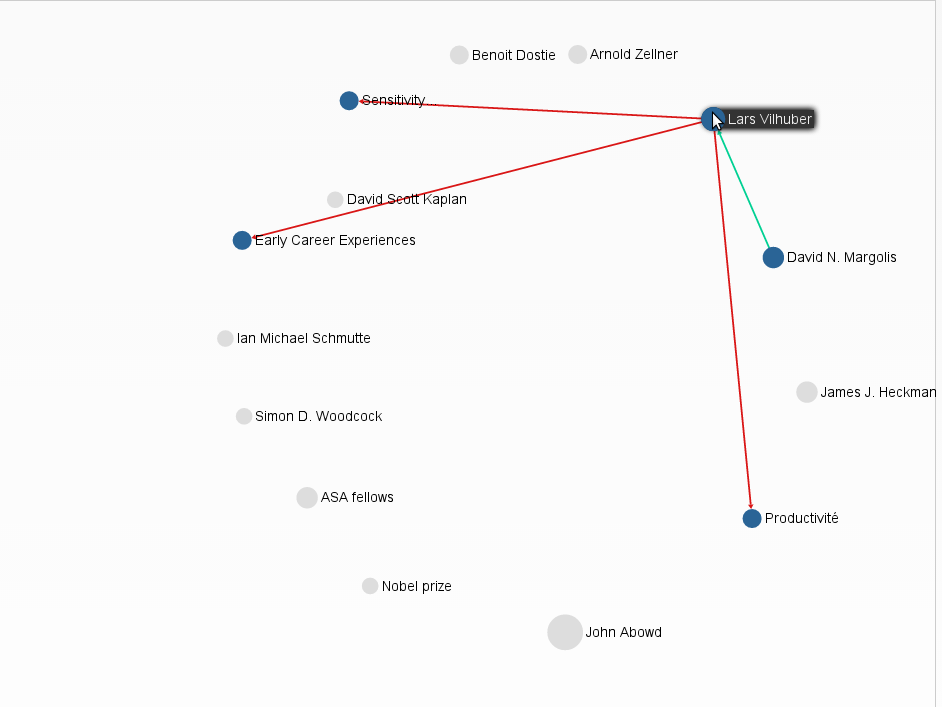
\includegraphics[width=0.9\textwidth]{web-interface-pvi26}
\end{figure}
\clearpage

\section{Future work}
\label{sec:future_work}
Already present in the \repec~ network are citation links (linking papers among themselves). This work links in with CED$^2$AR work (citations) and other efforts for linking papers and articles to the data used for (empirical) papers. Establishing such links can be represented by a tripartite graph:

\begin{figure}[ht]
\caption{Authorship with theses, data}\label{fig:tripartite}
% from http://tex.stackexchange.com/questions/15088/bipartite-graphs

\begin{tikzpicture}[thick,
  >=triangle 60,              % Nice arrows; your taste may be different	
  every node/.style={draw,circle},
  fsnode/.style={fill=ncentity},
  ssnode/.style={fill=lcauthor!25},
  every fit/.style={ellipse,draw,inner sep=2pt,text width=2cm},
  ->,shorten >= 3pt,shorten <= 3pt
]

\begin{scope}[start chain=going below,node distance=7mm]
\foreach \i/\dataname in {1/CPS,2/LEHD,3/QWI,4/National QWI}
  \node[fsnode,on chain] (d\i) [label=left:  \dataname] {};
\end{scope}


% the vertices of U
\begin{scope}[xshift=4cm,start chain=going below,node distance=7mm]
\foreach \i/\nodename in {1/Gross Flows,2/Nat.Estimates,3/Sorting}
  \node[fsnode,on chain] (p\i) [label=above: \i] {};
\end{scope}

% the vertices of T
\begin{scope}[xshift=4cm,yshift=-4cm,start chain=going below,node distance=7mm]
\foreach \i/\nodename in {1/pab175,2/pma385,3/pvi26,4/psc351}
  \node[fsnode,on chain] (t\i) [label=left: \href{https://genealogy.repec.org/pages/\nodename .html}{\nodename thesis}] {};
\end{scope}

%
% the vertices of V
\begin{scope}[xshift=8cm,yshift=-0.5cm,start chain=going below,node distance=7mm]
\foreach \i/\repecid  in {1/pab175,2/pze9,3/pvi26,4/psc351,5/pkr29,6/pma385,7/ple92,8/unknown}
  \node[ssnode,on chain] (s\i) [label=right: \i\ \href{http://ideas.repec.org/f/\repecid .html}{\repecid}] {};
\end{scope}


% the set U
\node [lcauthor,fit=(p1) (p3),label=above:$Papers$] {};
% the set V
\node [ncentity,fit=(s1) (s8),label=above:$Authors$] {};
% the set T
\node [lcauthor,fit=(t1) (t4),label=below:$Thesis$] {};
% the set D
\node [lcuse,fit=(d1) (d4),label=above:$Data$] {};

% the edges
\draw [densely dotted] (p1) -- (s1);
\draw [densely dotted] (p1) -- (s2);
\draw [densely dotted] (p2) -- (s1);
\draw [densely dotted] (p2) -- (s3);
\draw [densely dotted] (p3) -- (s1);
\draw [densely dotted] (p3) -- (s4);
\draw [densely dotted] (p3) -- (s5);
\draw [densely dotted] (p3) -- (s8);
% for the theses
% the edges
\draw [densely dotted] (t1) -- (s1);
\draw [densely dotted] (t2) -- (s4);
\draw [densely dotted] (t3) -- (s5);
\draw [densely dotted] (t4) -- (s4);
\draw [densely dotted] (s2) -- (t1);
\draw [densely dotted] (s3) -- (t1);
\draw [densely dotted] (s1) -- (t2);
\draw [densely dotted] (s4) -- (t3);
\draw [densely dotted] (s6) -- (t3);
\draw [densely dotted] (s1) -- (t4);
% data
\path (d1) to node [lcuse, yshift=-1em, above, draw=none] {used} (p1);
\draw [lcuse] (p1) -- (d1);
\draw [lcuse] (p2) -- (d3);
\draw [lcuse] (p2) -- (d1);
\draw [lcuse] (d3) -- (d2);
\draw [lcuse] (d4) -- (d3);
\draw [lcuse] (p3) -- (d2);
\draw [lcuse] (t4) -- (d2);
\path (d4) to node [lcadvisor,below, rotate=30, yshift=2em, draw=none] {generatedBy} (p2);
\draw [lcadvisor] (d4) -- (p2);


\end{tikzpicture}

\end{figure}
This will ultimately allow to attribute authorship for certain datasets in a clear fashion, which is currently not usual in the social sciences.\footnote{See ICPSR examples, however.} For an example, see Figure~\ref{fig:tripartite-hilite}.

\begin{figure}[ht]
\caption{Authorship of data}\label{fig:tripartite-hilite}
% from http://tex.stackexchange.com/questions/15088/bipartite-graphs

\begin{tikzpicture}[thick,
  >=triangle 60,              % Nice arrows; your taste may be different	
  every node/.style={draw,circle},
  fsnode/.style={fill=ncentity},
  ssnode/.style={fill=lcauthor!25},
  every fit/.style={ellipse,draw,inner sep=2pt,text width=2cm},
  ->,shorten >= 3pt,shorten <= 3pt
]

\begin{scope}[start chain=going below,node distance=7mm]
\foreach \i/\dataname in {1/CPS,2/LEHD,3/QWI,4/National QWI}
  \node[fsnode,on chain] (d\i) [label=left:  \dataname] {};
\end{scope}


% the vertices of U
\begin{scope}[xshift=4cm,start chain=going below,node distance=7mm]
\foreach \i/\nodename in {1/Gross Flows,2/Nat.Estimates,3/Sorting}
  \node[fsnode,on chain] (p\i) [label=above: \i] {};
\end{scope}

% the vertices of T
\begin{scope}[xshift=4cm,yshift=-4cm,start chain=going below,node distance=7mm]
\foreach \i/\nodename in {1/pab175,2/pma385,3/pvi26,4/psc351}
  \node[fsnode,on chain] (t\i) [label=left: \href{https://genealogy.repec.org/pages/\nodename .html}{\nodename thesis}] {};
\end{scope}

%
% the vertices of V
\begin{scope}[xshift=8cm,yshift=-0.5cm,start chain=going below,node distance=7mm]
\foreach \i/\repecid  in {1/pab175,2/pze9,3/pvi26,4/psc351,5/pkr29,6/pma385,7/ple92,8/unknown}
  \node[ssnode,on chain] (s\i) [label=right: \i\ \href{http://ideas.repec.org/f/\repecid .html}{\repecid}] {};
\end{scope}


% the set U
\node [lcauthor,fit=(p1) (p3),label=above:$Papers$] {};
% the set V
\node [ncentity,fit=(s1) (s8),label=above:$Authors$] {};
% the set T
\node [lcauthor,fit=(t1) (t4),label=below:$Thesis$] {};
% the set D
\node [fit=(d1) (d4),label=above:$Data$] {};

% the edges
\draw [dotted] (p1) -- (s1);
\draw [dotted] (p1) -- (s2);
\draw [lcauthor, ultra thick] (p2) -- (s1);
\draw [lcauthor, ultra thick] (p2) -- (s3);
\draw [dotted] (p3) -- (s1);
\draw [dotted] (p3) -- (s4);
\draw [dotted] (p3) -- (s5);
\draw [dotted] (p3) -- (s8);
% for the theses
% the edges
\draw [dotted] (t1) -- (s1);
\draw [dotted] (t2) -- (s4);
\draw [dotted] (t3) -- (s5);
\draw [dotted] (t4) -- (s4);
\draw [dotted] (s2) -- (t1);
\draw [dotted] (s3) -- (t1);
\draw [dotted] (s1) -- (t2);
\draw [dotted] (s4) -- (t3);
\draw [dotted] (s6) -- (t3);
\draw [dotted] (s1) -- (t4);
% data
\path (d1) to node [dotted, yshift=-1em, above, draw=none] {used} (p1);
\draw [dotted] (p1) -- (d1);
\draw [dotted] (p2) -- (d3);
\draw [dotted] (p2) -- (d1);
\draw [dotted] (d3) -- (d2);
\draw [dotted] (d4) -- (d3);
\draw [dotted] (p3) -- (d2);
\draw [dotted] (t4) -- (d2);
\path (d4) to node [lcadvisor,below, rotate=30, yshift=2em, draw=none] {generatedBy} (p2);
\draw [lcadvisor, ultra thick] (d4) -- (p2);


\end{tikzpicture}

\end{figure}


\end{document}
